%%%%%% CMB-S4 Experimental Approach Chapter  %%%%%%%%%%%%%%%%
 
\chapter{Experimental Approach}
%\renewcommand*\thesection{\arabic{section}}

\def\nnu{N_{\mathrm eff}}
\def\gtrsim{\raise-.75ex\hbox{$\buildrel>\over\sim$}}
%%%%%%%%%%%%%%%%%%%%%%%%%%%%%%%%%%%%%%%%%%%%%%%%%%%%%%%%%%%
%%%%%%%%%%%%%%%%%%%%%%%%%%%%%%%%%%%%%%%%%%%%%%%%%%%%%%%%%%%
%%%%%%%%%%%%%%%%%%%%%%%%%%%%%%%%%%%%%%%%%%%%%%%%%%%%%%%%%%%
%%%%%%%%%%%%%%%%%%%%%%%%%%%%%%%%%%%%%%%%%%%%%%%%%%%%%%%%%%%

\section{Introduction}


\begin{figure}[!h]
\centering 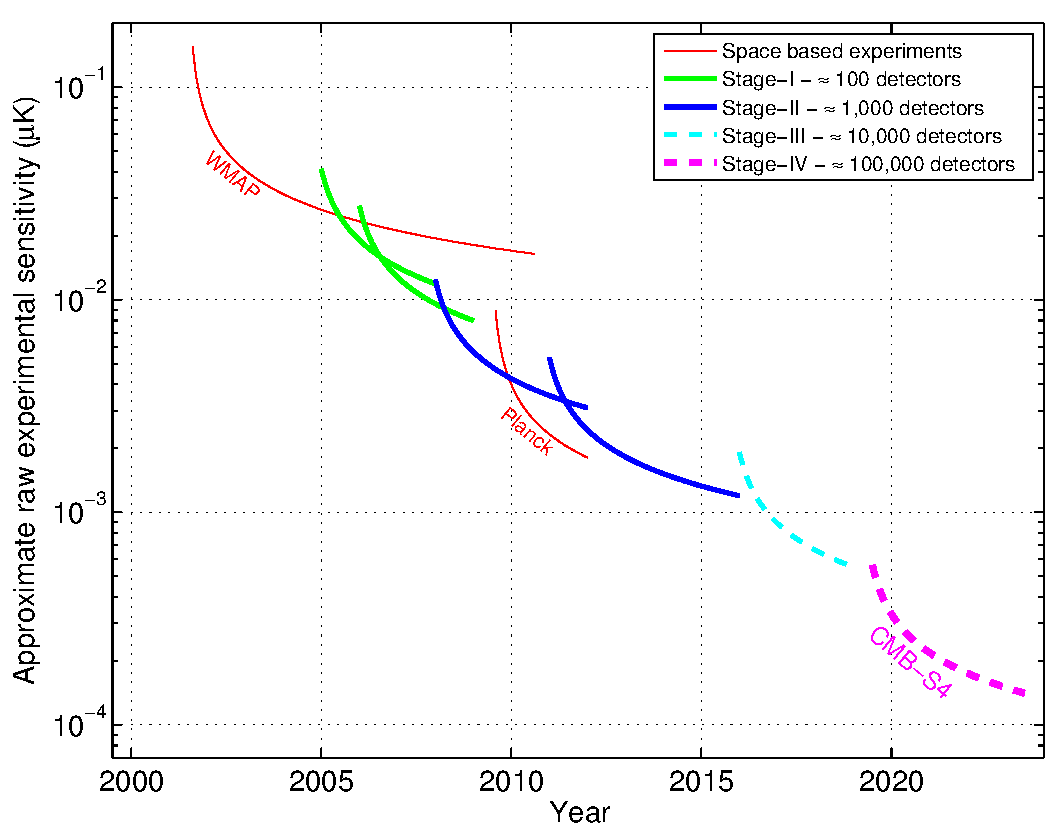
\includegraphics[width=0.6\textwidth]{Intro/expt_progress.pdf}
\caption{Plot illustrating the evolution of the raw sensitivity of CMB
  experiments, which scales as the total number of
  bolometers. Ground-based CMB experiments are classified into Stages
  with Stage II experiments having $O$(1000) detectors, Stage III
  experiments having $O$(10,000) detectors, and a Stage IV experiment
  (such as \cmbexp) having $O$(100,000) detectors. Figure from Snowmass  CF5
  Neutrino planning document.}
\label{fig:expt_progress}
\end{figure}

     
    \begin{figure}[ht]
\centering 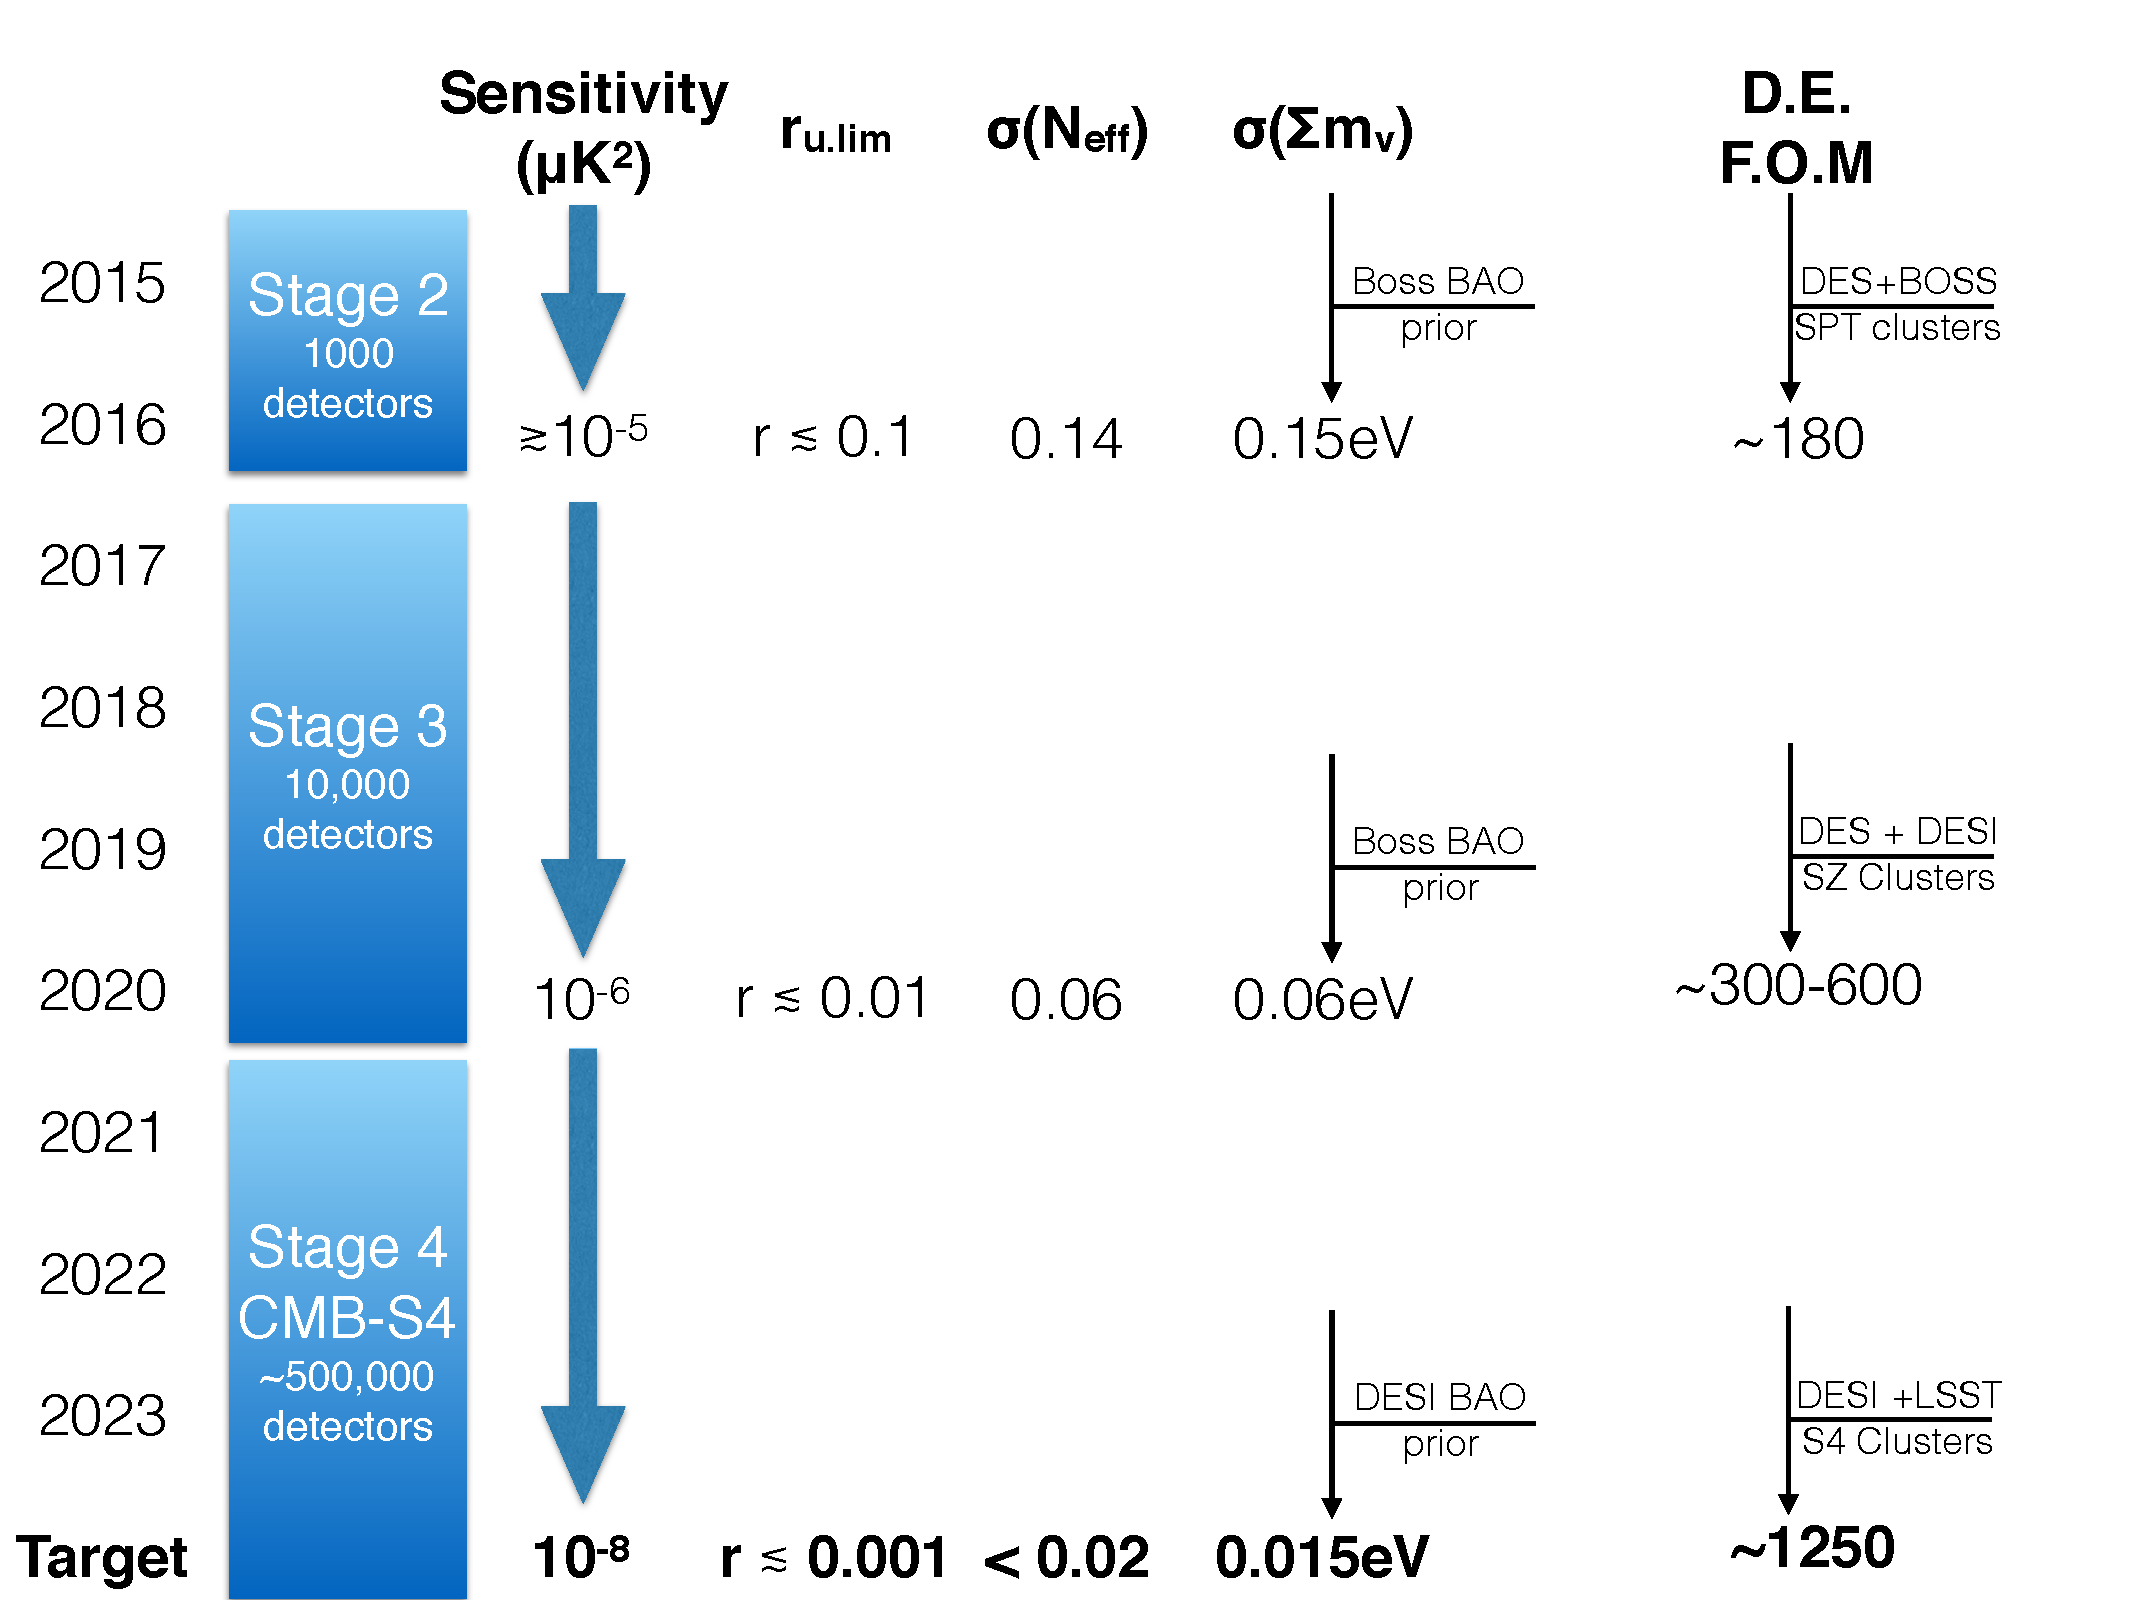
\includegraphics[width=0.95\textwidth]{Intro/Fig-FlowChart1_v1.pdf}
\caption{Schematic timeline of evolution of Stage 3 and CMB-S4 
sensitivity in $\mu$K$^2$ and the expected improvement in a few of the key cosmological parameters.}
\label{fig:science_timeline}
\end{figure} 

Experiment design from science goals

     
     - depth
     
     - sky area
     
     - resolution
     
          - ell space coverage
     
     -frequency coverage


\section{Complementarity of Ground and Space}

\section{Detector Arrays}
     
     - Superconducting Arrays
          
     - TES

\section{Multiplexer technologies}

\section{Telescopes and Optics}

     - Polarization modulators

\section{Sites}

     - Chile + Pole

     - Northern Site
     
     
%\bibliography{cmbs4}

%%
%% Populate the .bib file with entries from SPIRES Bibtex (preferred)
%% or ADS Bibtex (if no SPIRES entry).
%%  SPIRES will also supply the CITATION line information; please include it.
%%


